\chapter{EPR ``theorem''}
\label{chap:epr}
The first chapter of this thesis will be concerned with the so called ``EPR paradox''. In their famous article of 1935 \cite{PhysRev.47.777} Albert Einstein, Boris Podolsky and Natan Rosen (EPR) presented a strong logical reasoning against (the Copenhagen interpretation of) quantum mechanics. Starting from few reasonable assumptions on the locality of physical processes, some form of realism and predictions taken from quantum mechanics they derive a clear conclusion: Quantum mechanics can at most be regarded as a statistical description of ensembles of physical systems. Single systems contain more information than the theory incorporates.%comment on by-products of their argument.
%We prefer to use the word ``theorem'' to refer to this result to remark its


\section{Perfect correlations in systems of two spin-1/2 particles}
\label{sec:two-spin1/2}

\begin{figure}
  \centering
  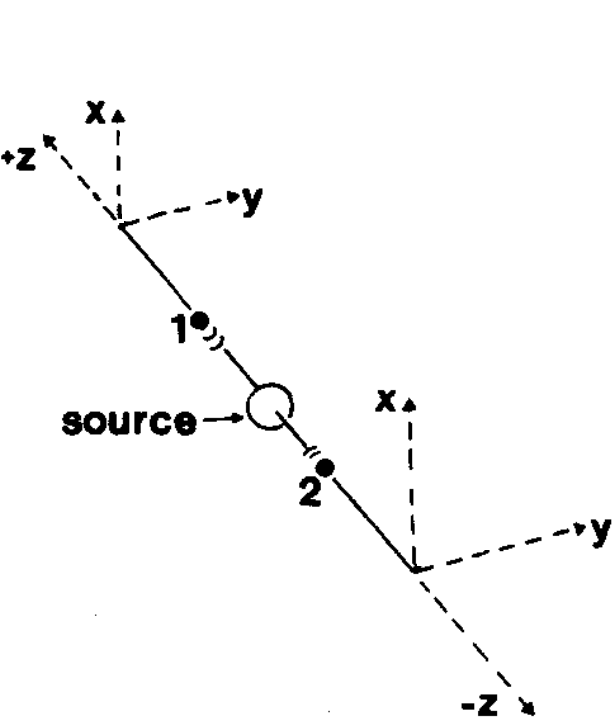
\includegraphics[width=0.275\textwidth]{Mainmatter/Chapter1/eprb-gedankenexperiment.png}
  \caption{The Bohm gedankenexperiment. Credits \cite{:/content/aapt/journal/ajp/58/12/10.1119/1.16243}.}
  \label{fig:eprb-gedankenexperiment}
\end{figure}

In this section we will present some aspects of the quantum mechanical description of systems composed of two spin-1/2 particles. In particular we will show that there exist situations for which quantum mechanics predicts perfect correlation between the results of measurements performed on the two particles. We will also see that such correlations are independent of where and when the two measurements are performed.%is it clear enough that the two measurements are made on the two particles separately?

Consider for instance two spin-1/2 particles emitted at a source and propagating in opposite directions along the $\mathbf{\hat{z}}$ axis (see Fig. \ref{fig:eprb-gedankenexperiment}).  Each particle then enters an apparatus (e.g. a Stern-Gerlach magnet) that can measure either the $S_x$ or $S_y$ spin component. Suppose that the two particles are emitted in the state with total spin equal to $0$, that is:
\begin{equation}
  |\chi\rangle = \frac{1}{\sqrt{2}} \left( |+\rangle_1 |-\rangle_2 - |-\rangle_1 |+\rangle_2 \right)
  \label{eq:singlet-state}
\end{equation}
where the vectors $|+\rangle_i$ and $|-\rangle_i$ represent, respectively, states of spin up and down along an arbitrary direction $\mathbf{\hat{n}} = \mathbf{\hat{x}}, \mathbf{\hat{y}}, \mathbf{\hat{z}}$ for particle $i = 1, 2$. The state (\ref{eq:singlet-state}) is such as to take the same form independently of $\mathbf{\hat{n}}$, thus no ambiguity arises from omitting the direction $\mathbf{\hat{n}}$ in the notation (see Appendix \ref{app:spin-predictions} for a proof of this statement). This last statement also allows us to easily see that if the two measuring apparatuses happen to be oriented in the same direction, that is if they both measure either the $S_x$ or $S_y$ spin component, then the spins of the two particles will be found to have opposite sign.%is the notation confusing here?

\begin{remark}
  Notice that the perfect correlation we have predicted in this section are independent on the time order with which we perform the two measurements as well as on the distance between the places where the two measuring apparatuses are located.%should I add something like: ``as long as the spin state doesn't change''?
\end{remark}

\begin{observation}
  The correlation between the results of measurements presented here is a peculiar trait of entanglement. Let us demonstrate that the state (\ref{eq:singlet-state}) is entangled. If it wasn't it could be written as:
\begin{equation*}
  |\chi\rangle = |u\rangle_1 |v\rangle_2,
\end{equation*}
since the couple $\left(|+\rangle_i, |-\rangle_i\right)$ is a basis for the spin space of particle $i$ we would have:
\begin{equation*}
  \begin{split}
    |u\rangle_1 &= a |+\rangle_1 + b |-\rangle_1,\\
    |v\rangle_2 &= c |+\rangle_2 + d |-\rangle_2
  \end{split}
\end{equation*}
for some $a, b, c$ and $d$, thus:
\begin{equation*}
  |\chi\rangle = a c |+\rangle_1 |+\rangle_2 + a d |+\rangle_1 |-\rangle_2 + b c |-\rangle_1 |+\rangle_2 + b d |-\rangle_1 |-\rangle_2.
\end{equation*}
Comparing this last equation with (\ref{eq:singlet-state}) we get:
\begin{equation*}
  \begin{split}
    a c &= b d = 0,\\
    a d &= 1,\\
    b c &= - 1
  \end{split}
\end{equation*}
which yield $0 = -1$. This absurd conclusion is removed admitting that the state (\ref{eq:singlet-state}) is entangled.
\end{observation}

\begin{observation}
  In this section we made use of labels for the two particles. This is for sure legitimate if the two particles are different but, with a slight change of the label's meaning, labels can be used in the case of identical particles too. It is in fact sufficient to regard 1 and 2 as labels of the measuring apparatus in which the particle is detected.%is some better explenation needed here?
\end{observation}


\section{The EPR argument}
\label{epr-argument}
In this section we will present the argument proposed by Einstein, Podolsky and Rosen \cite{PhysRev.47.777} to prove that quantum mechanics is incomplete.

\begin{note}
Throughout the presentation of the argument we will refer to the experimental conditions considered in the previous section.
\end{note}

Let us start by stating clearly all the assumptions on which the argument rests. The first of these is the prediction of quantum mechanics we have derived in the previous section, that is:
\begin{enumerate}
  %enumerated lists style
  \renewcommand{\theenumi}{\alph{enumi}}
  \renewcommand{\labelenumi}{(\theenumi)}
\item \label{itm:epr-perfect-correlation} \textit{Perfect correlation:} If the spins of the two particles are measured along the same direction, then the two spins will be found (with certainty) to have opposite sign (independently of the time order and spatial distance at which the two measurements are performed).
\end{enumerate}
We then assume the validity of the following (necessary) requirement for a theory to be complete:
\begin{enumerate}
  \setcounter{enumi}{1}
  %enumerated lists style
  \renewcommand{\theenumi}{\alph{enumi}}
  \renewcommand{\labelenumi}{(\theenumi)}
\item \label{itm:epr-completeness} \textit{Completeness:} ``Every element of the physical reality must have a counterpart in the [complete] physical theory.'' \cite{PhysRev.47.777}
\end{enumerate}
Where to identify the elements of the physical reality we assume the validity of the (sufficient) criterion that follows:
\begin{enumerate}
  \setcounter{enumi}{2}
  %enumerated lists style
  \renewcommand{\theenumi}{\alph{enumi}}
  \renewcommand{\labelenumi}{(\theenumi)}
\item \label{itm:epr-reality} \textit{Reality:} ``If, without in any way disturbing a system, we can predict with certainty (i.e. with probability equal to unity) the value of a physical quantity, then there exists an element of physical reality corresponding to this physical quantity.'' \cite{PhysRev.47.777}
\end{enumerate}
At last we assume that the two measuring apparatuses are very far form each other, thus, again in EPR's words \cite{PhysRev.47.777}:
\begin{enumerate}
  \setcounter{enumi}{3}
  %enumerated lists style
  \renewcommand{\theenumi}{\alph{enumi}}
  \renewcommand{\labelenumi}{(\theenumi)}
\item \label{itm:epr-locality} \textit{Locality:} ``Since at the time of measurement the two systems [(the two particles in our case)] no longer interact, no real change [\footnote{By ``real change'' we mean changes to the \textit{elements of the physical reality}}] can take place in the second system in consequence of anything that may be done to the first system.''
\end{enumerate}

The argument is then the following: Suppose a spin component, say $S_x$ ($S_y$), of particle 1 is measured at some time $t_1$, because of the perfect correlation assumption (\ref{itm:epr-perfect-correlation}), we know that if at some time $t_2 > t_1$ the same spin component of particle 2 is measured it will be found (with certainty) to have opposite sign. Locality, (\ref{itm:epr-locality}), ensures that the elements of physical reality associated to particle 2 have not changed as a consequence of the measurement performed on particle 1. Thus, by the reality assumption (\ref{itm:epr-reality}), there is an element of physical reality corresponding to the $S_x$ ($S_y$) physical quantity of particle 2. Using again (\ref{itm:epr-locality}) we can state that such element of physical reality existed before the measurement on particle 1 was performed. Exchanging the role of the two particles in the previous steps leads to the conclusion that there corresponds an element of physical reality also to the $S_x$ ($S_y$) physical quantity of particle 1, this element of physical reality too existed before \textit{any} measurement was performed. We have thus obtained that the results of the two measurements were predetermined. Since the quantum state considered, (\ref{eq:singlet-state}), does not determine the result of the two measurements, we conclude that the theory ignores the elements of reality we have found to exist and, by completeness (\ref{itm:epr-completeness}), must be considered incomplete. This completes the proof of the EPR ``theorem''.%is the final step clear enough or is it better to go Laloe's way? - is the S_y thing clear enough? - is it clear that the state considered at the beginning is the singlet one?

\begin{remark}
  It is worth noting here, as Laloë does in \cite{:/content/aapt/journal/ajp/69/6/10.1119/1.1356698}, that, since perfect correlation is observed only when the particles are in state (\ref{eq:singlet-state}), the elements of reality ignored by quantum mechanics cannot be attached to any object other than the two particles. We implicitly made use of this fact in the demonstration of the argument.
%  After noting that if we
%  As a matter of fact the argument
%  The possibility of attaching distinct elements of reality to the two (spatially separated) particles comes from what is sometimes called ``separability''.
%  We report here a quote from \cite{:/content/aapt/journal/ajp/69/6/10.1119/1.1356698} to summarize the situation: ``the basig belief of EPR is that regions of space...''
\end{remark}

\begin{observation}
  The original argument by Einstein, Podolsky and Rosen \cite{PhysRev.47.777} doesn't involve spin degrees of freedom. The correlation they exploit to carry out their demonstration is between positions and momenta of two particles. The version of the argument we have presented here is due to Bohm \cite{bohm1951quantum}.

  Another point in which the argument we have presented differs from that of EPR is the final part. Their argument goes through considerations about hypothetical measurements of incompatible observables while we jumped straight to the conclusion.

  Moreover, in the original article Einstein, Podolsky and Rosen assume (\ref{itm:epr-locality}) but do not specify how one can be assured that the two systems no longer interact. We have specified one such a way, namely bringing the two systems far from each other. That Einstein would have agreed with us on this ca be deduced from the following quote: ``But on one supposition we should, in my opinion, absolutely hold fast: the real factual situation of the system $S_2$ is independent of what is done with the system $S_1$, which is spatially separated from the former.'' \cite{schilpp1949albert}.%What did E. really mean by ``spatially separated''. Things would change if he meant space-like separation...
\end{observation}
